\documentclass[1p]{elsarticle_modified}
%\bibliographystyle{elsarticle-num}

%\usepackage[colorlinks]{hyperref}
%\usepackage{abbrmath_seonhwa} %\Abb, \Ascr, \Acal ,\Abf, \Afrak
\usepackage{amsfonts}
\usepackage{amssymb}
\usepackage{amsmath}
\usepackage{amsthm}
\usepackage{scalefnt}
\usepackage{amsbsy}
\usepackage{kotex}
\usepackage{caption}
\usepackage{subfig}
\usepackage{color}
\usepackage{graphicx}
\usepackage{xcolor} %% white, black, red, green, blue, cyan, magenta, yellow
\usepackage{float}
\usepackage{setspace}
\usepackage{hyperref}

\usepackage{tikz}
\usetikzlibrary{arrows}

\usepackage{multirow}
\usepackage{array} % fixed length table
\usepackage{hhline}

%%%%%%%%%%%%%%%%%%%%%
\makeatletter
\renewcommand*\env@matrix[1][\arraystretch]{%
	\edef\arraystretch{#1}%
	\hskip -\arraycolsep
	\let\@ifnextchar\new@ifnextchar
	\array{*\c@MaxMatrixCols c}}
\makeatother %https://tex.stackexchange.com/questions/14071/how-can-i-increase-the-line-spacing-in-a-matrix
%%%%%%%%%%%%%%%

\usepackage[normalem]{ulem}

\newcommand{\msout}[1]{\ifmmode\text{\sout{\ensuremath{#1}}}\else\sout{#1}\fi}
%SOURCE: \msout is \stkout macro in https://tex.stackexchange.com/questions/20609/strikeout-in-math-mode

\newcommand{\cancel}[1]{
	\ifmmode
	{\color{red}\msout{#1}}
	\else
	{\color{red}\sout{#1}}
	\fi
}

\newcommand{\add}[1]{
	{\color{blue}\uwave{#1}}
}

\newcommand{\replace}[2]{
	\ifmmode
	{\color{red}\msout{#1}}{\color{blue}\uwave{#2}}
	\else
	{\color{red}\sout{#1}}{\color{blue}\uwave{#2}}
	\fi
}

\newcommand{\Sol}{\mathcal{S}} %segment
\newcommand{\D}{D} %diagram
\newcommand{\A}{\mathcal{A}} %arc


%%%%%%%%%%%%%%%%%%%%%%%%%%%%%5 test

\def\sl{\operatorname{\textup{SL}}(2,\Cbb)}
\def\psl{\operatorname{\textup{PSL}}(2,\Cbb)}
\def\quan{\mkern 1mu \triangleright \mkern 1mu}

\theoremstyle{definition}
\newtheorem{thm}{Theorem}[section]
\newtheorem{prop}[thm]{Proposition}
\newtheorem{lem}[thm]{Lemma}
\newtheorem{ques}[thm]{Question}
\newtheorem{cor}[thm]{Corollary}
\newtheorem{defn}[thm]{Definition}
\newtheorem{exam}[thm]{Example}
\newtheorem{rmk}[thm]{Remark}
\newtheorem{alg}[thm]{Algorithm}

\newcommand{\I}{\sqrt{-1}}
\begin{document}

%\begin{frontmatter}
%
%\title{Boundary parabolic representations of knots up to 8 crossings}
%
%%% Group authors per affiliation:
%\author{Yunhi Cho} 
%\address{Department of Mathematics, University of Seoul, Seoul, Korea}
%\ead{yhcho@uos.ac.kr}
%
%
%\author{Seonhwa Kim} %\fnref{s_kim}}
%\address{Center for Geometry and Physics, Institute for Basic Science, Pohang, 37673, Korea}
%\ead{ryeona17@ibs.re.kr}
%
%\author{Hyuk Kim}
%\address{Department of Mathematical Sciences, Seoul National University, Seoul 08826, Korea}
%\ead{hyukkim@snu.ac.kr}
%
%\author{Seokbeom Yoon}
%\address{Department of Mathematical Sciences, Seoul National University, Seoul, 08826,  Korea}
%\ead{sbyoon15@snu.ac.kr}
%
%\begin{abstract}
%We find all boundary parabolic representation of knots up to 8 crossings.
%
%\end{abstract}
%\begin{keyword}
%    \MSC[2010] 57M25 
%\end{keyword}
%
%\end{frontmatter}

%\linenumbers
%\tableofcontents
%
\newcommand\colored[1]{\textcolor{white}{\rule[-0.35ex]{0.8em}{1.4ex}}\kern-0.8em\color{red} #1}%
%\newcommand\colored[1]{\textcolor{white}{ #1}\kern-2.17ex	\textcolor{white}{ #1}\kern-1.81ex	\textcolor{white}{ #1}\kern-2.15ex\color{red}#1	}

{\Large $\underline{12a_{0637}~(K12a_{0637})}$}

\setlength{\tabcolsep}{10pt}
\renewcommand{\arraystretch}{1.6}
\vspace{1cm}\begin{tabular}{m{100pt}>{\centering\arraybackslash}m{274pt}}
\multirow{5}{120pt}{
	\centering
	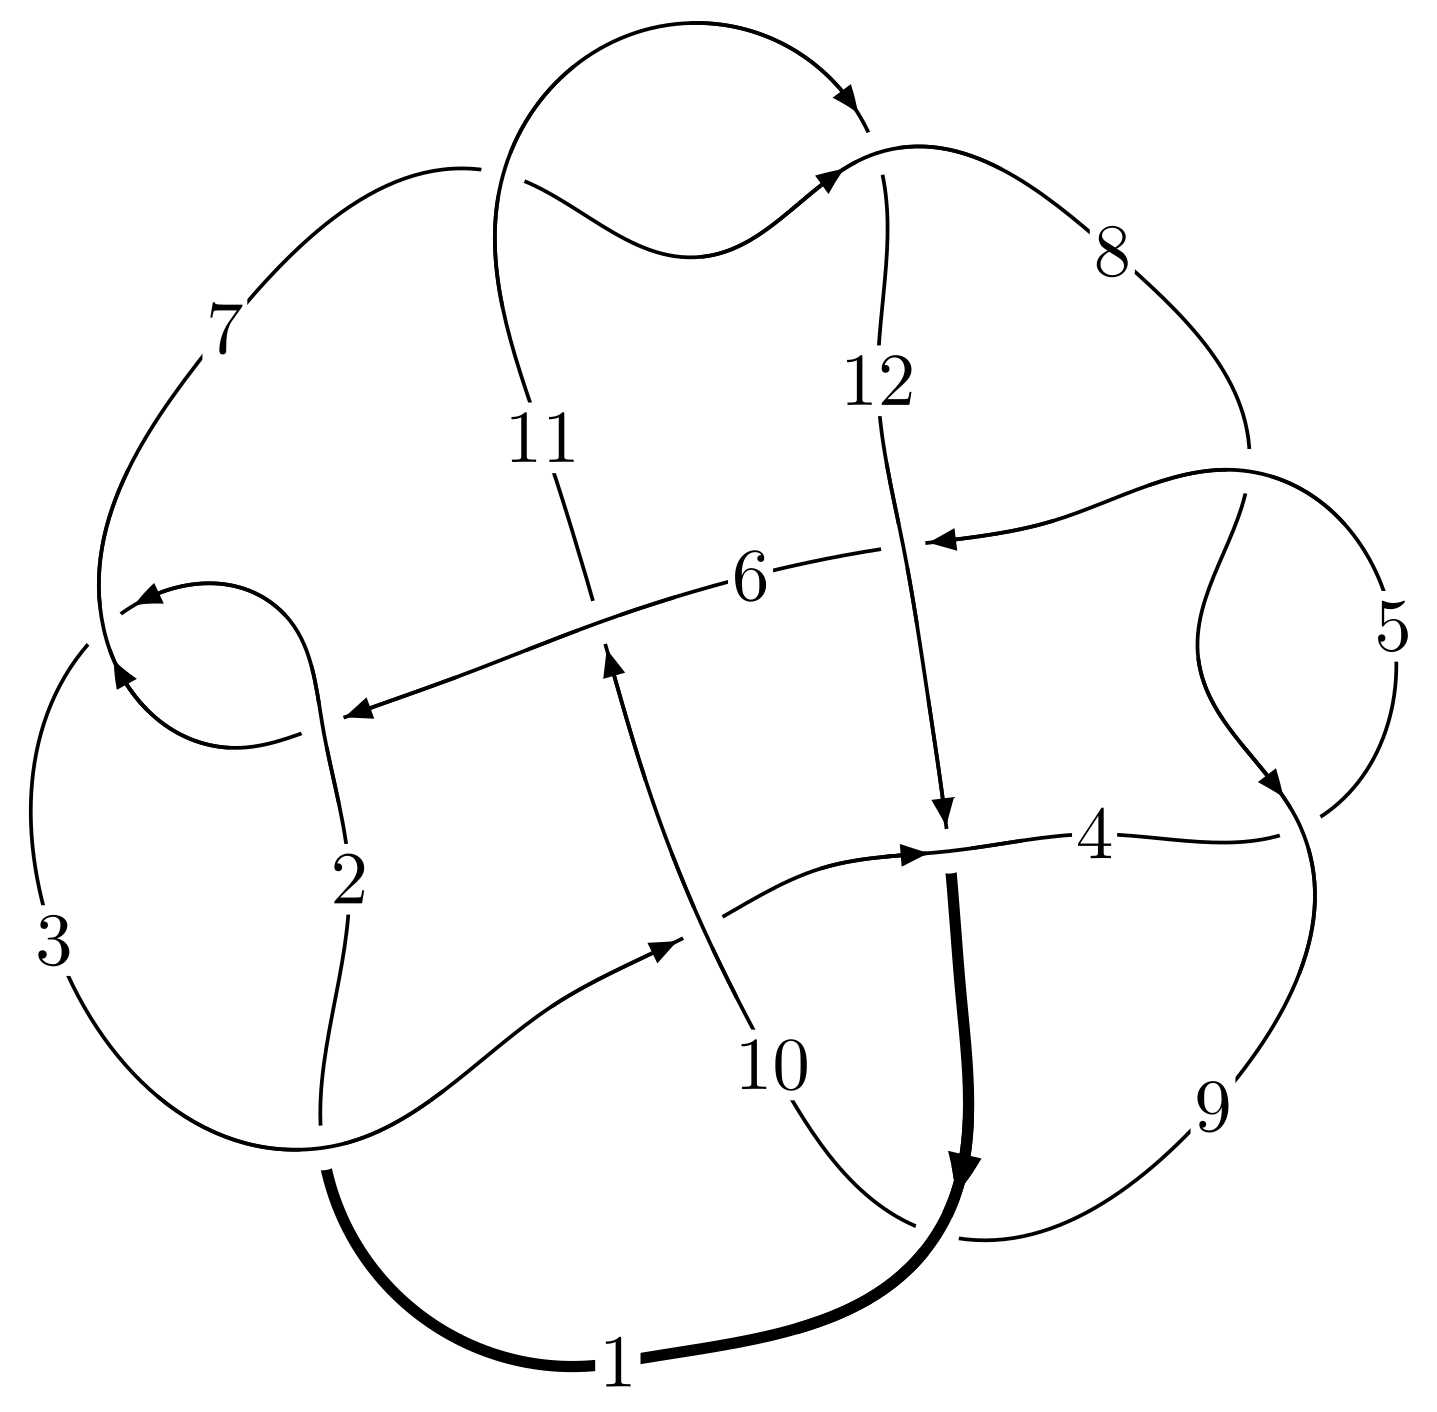
\includegraphics[width=112pt]{../../../GIT/diagram.site/Diagrams/png/1438_12a_0637.png}\\
\ \ \ A knot diagram\footnotemark}&
\allowdisplaybreaks
\textbf{Linearized knot diagam} \\
\cline{2-2}
 &
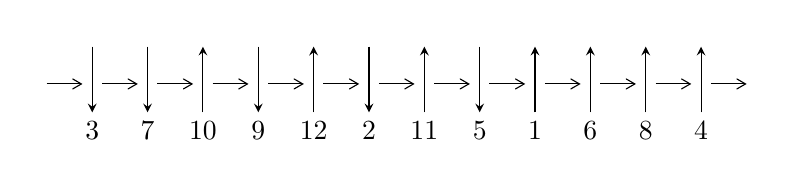
\begin{tikzpicture}[x=20pt, y=17pt]
	% nodes
	\node (C0) at (0, 0) {};
	\node (C1) at (1, 0) {};
	\node (C1U) at (1, +1) {};
	\node (C1D) at (1, -1) {3};

	\node (C2) at (2, 0) {};
	\node (C2U) at (2, +1) {};
	\node (C2D) at (2, -1) {7};

	\node (C3) at (3, 0) {};
	\node (C3U) at (3, +1) {};
	\node (C3D) at (3, -1) {10};

	\node (C4) at (4, 0) {};
	\node (C4U) at (4, +1) {};
	\node (C4D) at (4, -1) {9};

	\node (C5) at (5, 0) {};
	\node (C5U) at (5, +1) {};
	\node (C5D) at (5, -1) {12};

	\node (C6) at (6, 0) {};
	\node (C6U) at (6, +1) {};
	\node (C6D) at (6, -1) {2};

	\node (C7) at (7, 0) {};
	\node (C7U) at (7, +1) {};
	\node (C7D) at (7, -1) {11};

	\node (C8) at (8, 0) {};
	\node (C8U) at (8, +1) {};
	\node (C8D) at (8, -1) {5};

	\node (C9) at (9, 0) {};
	\node (C9U) at (9, +1) {};
	\node (C9D) at (9, -1) {1};

	\node (C10) at (10, 0) {};
	\node (C10U) at (10, +1) {};
	\node (C10D) at (10, -1) {6};

	\node (C11) at (11, 0) {};
	\node (C11U) at (11, +1) {};
	\node (C11D) at (11, -1) {8};

	\node (C12) at (12, 0) {};
	\node (C12U) at (12, +1) {};
	\node (C12D) at (12, -1) {4};
	\node (C13) at (13, 0) {};

	% arrows
	\draw[->,>={angle 60}]
	(C0) edge (C1) (C1) edge (C2) (C2) edge (C3) (C3) edge (C4) (C4) edge (C5) (C5) edge (C6) (C6) edge (C7) (C7) edge (C8) (C8) edge (C9) (C9) edge (C10) (C10) edge (C11) (C11) edge (C12) (C12) edge (C13) ;	\draw[->,>=stealth]
	(C1U) edge (C1D) (C2U) edge (C2D) (C3D) edge (C3U) (C4U) edge (C4D) (C5D) edge (C5U) (C6U) edge (C6D) (C7D) edge (C7U) (C8U) edge (C8D) (C9D) edge (C9U) (C10D) edge (C10U) (C11D) edge (C11U) (C12D) edge (C12U) ;
	\end{tikzpicture} \\
\hhline{~~} \\& 
\textbf{Solving Sequence} \\ \cline{2-2} 
 &
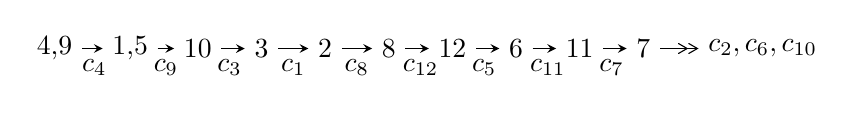
\begin{tikzpicture}[x=23pt, y=7pt]
	% node
	\node (A0) at (-1/8, 0) {4,9};
	\node (A1) at (17/16, 0) {1,5};
	\node (A2) at (17/8, 0) {10};
	\node (A3) at (25/8, 0) {3};
	\node (A4) at (33/8, 0) {2};
	\node (A5) at (41/8, 0) {8};
	\node (A6) at (49/8, 0) {12};
	\node (A7) at (57/8, 0) {6};
	\node (A8) at (65/8, 0) {11};
	\node (A9) at (73/8, 0) {7};
	\node (C1) at (1/2, -1) {$c_{4}$};
	\node (C2) at (13/8, -1) {$c_{9}$};
	\node (C3) at (21/8, -1) {$c_{3}$};
	\node (C4) at (29/8, -1) {$c_{1}$};
	\node (C5) at (37/8, -1) {$c_{8}$};
	\node (C6) at (45/8, -1) {$c_{12}$};
	\node (C7) at (53/8, -1) {$c_{5}$};
	\node (C8) at (61/8, -1) {$c_{11}$};
	\node (C9) at (69/8, -1) {$c_{7}$};
	\node (A10) at (11, 0) {$c_{2},c_{6},c_{10}$};

	% edge
	\draw[->,>=stealth]	
	(A0) edge (A1) (A1) edge (A2) (A2) edge (A3) (A3) edge (A4) (A4) edge (A5) (A5) edge (A6) (A6) edge (A7) (A7) edge (A8) (A8) edge (A9) ;
	\draw[->>,>={angle 60}]	
	(A9) edge (A10);
\end{tikzpicture} \\ 

\end{tabular} \\

\footnotetext{
The image of knot diagram is generated by the software ``\textbf{Draw programme}" developed by Andrew Bartholomew(\url{http://www.layer8.co.uk/maths/draw/index.htm\#Running-draw}), where we modified some parts for our purpose(\url{https://github.com/CATsTAILs/LinksPainter}).
}\phantom \\ \newline 
\centering \textbf{Ideals for irreducible components\footnotemark of $X_{\text{par}}$} 
 
\begin{align*}
I^u_{1}&=\langle 
-7.80686\times10^{608} u^{135}+4.59267\times10^{609} u^{134}+\cdots+3.53132\times10^{611} b+7.99940\times10^{610},\\
\phantom{I^u_{1}}&\phantom{= \langle  }-1.21400\times10^{609} u^{135}-1.85289\times10^{611} u^{134}+\cdots+1.45844\times10^{614} a-4.86124\times10^{614},\\
\phantom{I^u_{1}}&\phantom{= \langle  }u^{136}-5 u^{135}+\cdots-1764 u-392\rangle \\
I^u_{2}&=\langle 
3127351 u^{18}-1101560 u^{17}+\cdots+3308497 b-3526485,\\
\phantom{I^u_{2}}&\phantom{= \langle  }4211238 u^{18}-9238417 u^{17}+\cdots+3308497 a+6322815,\;u^{19}- u^{18}+\cdots-11 u^2-1\rangle \\
I^u_{3}&=\langle 
b,\;a+u,\;u^2- u+1\rangle \\
\\
\end{align*}
\raggedright * 3 irreducible components of $\dim_{\mathbb{C}}=0$, with total 157 representations.\\
\footnotetext{All coefficients of polynomials are rational numbers. But the coefficients are sometimes approximated in decimal forms when there is not enough margin.}
\newpage
\renewcommand{\arraystretch}{1}
\centering \section*{I. $I^u_{1}= \langle -7.81\times10^{608} u^{135}+4.59\times10^{609} u^{134}+\cdots+3.53\times10^{611} b+8.00\times10^{610},\;-1.21\times10^{609} u^{135}-1.85\times10^{611} u^{134}+\cdots+1.46\times10^{614} a-4.86\times10^{614},\;u^{136}-5 u^{135}+\cdots-1764 u-392 \rangle$}
\flushleft \textbf{(i) Arc colorings}\\
\begin{tabular}{m{7pt} m{180pt} m{7pt} m{180pt} }
\flushright $a_{4}=$&$\begin{pmatrix}1\\0\end{pmatrix}$ \\
\flushright $a_{9}=$&$\begin{pmatrix}0\\u\end{pmatrix}$ \\
\flushright $a_{1}=$&$\begin{pmatrix}8.32400\times10^{-6} u^{135}+0.00127046 u^{134}+\cdots+11.7711 u+3.33319\\0.00221075 u^{135}-0.0130055 u^{134}+\cdots+2.35289 u-0.226527\end{pmatrix}$ \\
\flushright $a_{5}=$&$\begin{pmatrix}1\\u^2\end{pmatrix}$ \\
\flushright $a_{10}=$&$\begin{pmatrix}-0.00320519 u^{135}+0.0124770 u^{134}+\cdots-18.1541 u-2.63362\\0.00190447 u^{135}-0.0132405 u^{134}+\cdots+4.84713 u+1.75434\end{pmatrix}$ \\
\flushright $a_{3}=$&$\begin{pmatrix}0.00961782 u^{135}-0.0513213 u^{134}+\cdots+2.39397 u+4.01892\\0.00525886 u^{135}-0.0201863 u^{134}+\cdots-7.87142 u-0.761178\end{pmatrix}$ \\
\flushright $a_{2}=$&$\begin{pmatrix}-0.0132748 u^{135}+0.0673620 u^{134}+\cdots-21.5615 u-2.98098\\-0.000837063 u^{135}-0.00318599 u^{134}+\cdots+7.32115 u+1.47992\end{pmatrix}$ \\
\flushright $a_{8}=$&$\begin{pmatrix}u\\u^3+u\end{pmatrix}$ \\
\flushright $a_{12}=$&$\begin{pmatrix}-0.00220242 u^{135}+0.0142760 u^{134}+\cdots+9.41817 u+3.55971\\0.00221075 u^{135}-0.0130055 u^{134}+\cdots+2.35289 u-0.226527\end{pmatrix}$ \\
\flushright $a_{6}=$&$\begin{pmatrix}-0.00128220 u^{135}+0.0191494 u^{134}+\cdots-15.4030 u+2.71700\\-0.00302398 u^{135}+0.0113216 u^{134}+\cdots+5.21126 u+0.327390\end{pmatrix}$ \\
\flushright $a_{11}=$&$\begin{pmatrix}0.00108998 u^{135}-0.00277045 u^{134}+\cdots+8.16182 u+3.74680\\0.000603983 u^{135}-0.00470337 u^{134}+\cdots+1.35625 u-0.268539\end{pmatrix}$ \\
\flushright $a_{7}=$&$\begin{pmatrix}-0.00620299 u^{135}+0.0265644 u^{134}+\cdots+29.1434 u+7.44215\\0.00106340 u^{135}-0.00871337 u^{134}+\cdots+5.45011 u+0.321834\end{pmatrix}$\\&\end{tabular}
\flushleft \textbf{(ii) Obstruction class $= -1$}\\~\\
\flushleft \textbf{(iii) Cusp Shapes $= 0.00348385 u^{135}-0.0403883 u^{134}+\cdots+22.9816 u+11.3314$}\\~\\
\newpage\renewcommand{\arraystretch}{1}
\flushleft \textbf{(iv) u-Polynomials at the component}\newline \\
\begin{tabular}{m{50pt}|m{274pt}}
Crossings & \hspace{64pt}u-Polynomials at each crossing \\
\hline $$\begin{aligned}c_{1}\end{aligned}$$&$\begin{aligned}
&u^{136}+52 u^{135}+\cdots+9209 u+529
\end{aligned}$\\
\hline $$\begin{aligned}c_{2},c_{6}\end{aligned}$$&$\begin{aligned}
&u^{136}-2 u^{135}+\cdots-89 u-23
\end{aligned}$\\
\hline $$\begin{aligned}c_{3}\end{aligned}$$&$\begin{aligned}
&u^{136}+7 u^{135}+\cdots-20 u-1
\end{aligned}$\\
\hline $$\begin{aligned}c_{4},c_{8}\end{aligned}$$&$\begin{aligned}
&u^{136}+5 u^{135}+\cdots+1764 u-392
\end{aligned}$\\
\hline $$\begin{aligned}c_{5}\end{aligned}$$&$\begin{aligned}
&u^{136}-3 u^{135}+\cdots-10733 u+829
\end{aligned}$\\
\hline $$\begin{aligned}c_{7},c_{11}\end{aligned}$$&$\begin{aligned}
&u^{136}-3 u^{135}+\cdots-5775 u+244
\end{aligned}$\\
\hline $$\begin{aligned}c_{9}\end{aligned}$$&$\begin{aligned}
&u^{136}-4 u^{135}+\cdots-59182 u-17287
\end{aligned}$\\
\hline $$\begin{aligned}c_{10}\end{aligned}$$&$\begin{aligned}
&u^{136}+4 u^{135}+\cdots+113947 u-42193
\end{aligned}$\\
\hline $$\begin{aligned}c_{12}\end{aligned}$$&$\begin{aligned}
&u^{136}+15 u^{135}+\cdots-36 u+8
\end{aligned}$\\
\hline
\end{tabular}\\~\\
\newpage\renewcommand{\arraystretch}{1}
\flushleft \textbf{(v) Riley Polynomials at the component}\newline \\
\begin{tabular}{m{50pt}|m{274pt}}
Crossings & \hspace{64pt}Riley Polynomials at each crossing \\
\hline $$\begin{aligned}c_{1}\end{aligned}$$&$\begin{aligned}
&y^{136}+68 y^{135}+\cdots+1258572891 y+279841
\end{aligned}$\\
\hline $$\begin{aligned}c_{2},c_{6}\end{aligned}$$&$\begin{aligned}
&y^{136}-52 y^{135}+\cdots-9209 y+529
\end{aligned}$\\
\hline $$\begin{aligned}c_{3}\end{aligned}$$&$\begin{aligned}
&y^{136}+5 y^{135}+\cdots-32 y+1
\end{aligned}$\\
\hline $$\begin{aligned}c_{4},c_{8}\end{aligned}$$&$\begin{aligned}
&y^{136}+109 y^{135}+\cdots-1223824 y+153664
\end{aligned}$\\
\hline $$\begin{aligned}c_{5}\end{aligned}$$&$\begin{aligned}
&y^{136}-47 y^{135}+\cdots-19505819 y+687241
\end{aligned}$\\
\hline $$\begin{aligned}c_{7},c_{11}\end{aligned}$$&$\begin{aligned}
&y^{136}-113 y^{135}+\cdots-9614305 y+59536
\end{aligned}$\\
\hline $$\begin{aligned}c_{9}\end{aligned}$$&$\begin{aligned}
&y^{136}-42 y^{135}+\cdots+9263767506 y+298840369
\end{aligned}$\\
\hline $$\begin{aligned}c_{10}\end{aligned}$$&$\begin{aligned}
&y^{136}-30 y^{135}+\cdots-52468465753 y+1780249249
\end{aligned}$\\
\hline $$\begin{aligned}c_{12}\end{aligned}$$&$\begin{aligned}
&y^{136}-11 y^{135}+\cdots-1776 y+64
\end{aligned}$\\
\hline
\end{tabular}\\~\\
\newpage\flushleft \textbf{(vi) Complex Volumes and Cusp Shapes}
$$\begin{array}{c|c|c}  
\text{Solutions to }I^u_{1}& \I (\text{vol} + \sqrt{-1}CS) & \text{Cusp shape}\\
 \hline 
\begin{aligned}
u &= \phantom{-}0.981483 + 0.194710 I \\
a &= \phantom{-}0.487582 - 1.061820 I \\
b &= \phantom{-}0.684933 - 0.932359 I\end{aligned}
 & -3.02456 - 6.65628 I & \phantom{-0.000000 } 0 \\ \hline\begin{aligned}
u &= \phantom{-}0.981483 - 0.194710 I \\
a &= \phantom{-}0.487582 + 1.061820 I \\
b &= \phantom{-}0.684933 + 0.932359 I\end{aligned}
 & -3.02456 + 6.65628 I & \phantom{-0.000000 } 0 \\ \hline\begin{aligned}
u &= -0.302840 + 0.950578 I \\
a &= \phantom{-}1.44682 - 0.22641 I \\
b &= -0.296701 - 0.506353 I\end{aligned}
 & -0.76134 + 6.16481 I & \phantom{-0.000000 } 0 \\ \hline\begin{aligned}
u &= -0.302840 - 0.950578 I \\
a &= \phantom{-}1.44682 + 0.22641 I \\
b &= -0.296701 + 0.506353 I\end{aligned}
 & -0.76134 - 6.16481 I & \phantom{-0.000000 } 0 \\ \hline\begin{aligned}
u &= -0.979464 + 0.038146 I \\
a &= \phantom{-}1.046020 - 0.701042 I \\
b &= \phantom{-}0.722445 - 0.812577 I\end{aligned}
 & -1.52856 - 8.54158 I & \phantom{-0.000000 } 0 \\ \hline\begin{aligned}
u &= -0.979464 - 0.038146 I \\
a &= \phantom{-}1.046020 + 0.701042 I \\
b &= \phantom{-}0.722445 + 0.812577 I\end{aligned}
 & -1.52856 + 8.54158 I & \phantom{-0.000000 } 0 \\ \hline\begin{aligned}
u &= \phantom{-}0.151638 + 1.012050 I \\
a &= \phantom{-}0.161145 - 0.868688 I \\
b &= \phantom{-}3.41324 + 0.54552 I\end{aligned}
 & \phantom{-}3.12305 + 2.06608 I & \phantom{-0.000000 } 0 \\ \hline\begin{aligned}
u &= \phantom{-}0.151638 - 1.012050 I \\
a &= \phantom{-}0.161145 + 0.868688 I \\
b &= \phantom{-}3.41324 - 0.54552 I\end{aligned}
 & \phantom{-}3.12305 - 2.06608 I & \phantom{-0.000000 } 0 \\ \hline\begin{aligned}
u &= -0.979982 + 0.309514 I \\
a &= -0.25551 - 1.41166 I \\
b &= \phantom{-}0.136556 - 0.747463 I\end{aligned}
 & \phantom{-}3.04388 - 0.52509 I & \phantom{-0.000000 } 0 \\ \hline\begin{aligned}
u &= -0.979982 - 0.309514 I \\
a &= -0.25551 + 1.41166 I \\
b &= \phantom{-}0.136556 + 0.747463 I\end{aligned}
 & \phantom{-}3.04388 + 0.52509 I & \phantom{-0.000000 } 0\\
 \hline 
 \end{array}$$\newpage$$\begin{array}{c|c|c}  
\text{Solutions to }I^u_{1}& \I (\text{vol} + \sqrt{-1}CS) & \text{Cusp shape}\\
 \hline 
\begin{aligned}
u &= \phantom{-}0.914350 + 0.469337 I \\
a &= \phantom{-}0.15902 - 1.71081 I \\
b &= -0.083275 - 0.829333 I\end{aligned}
 & \phantom{-}2.05985 + 5.50935 I & \phantom{-0.000000 } 0 \\ \hline\begin{aligned}
u &= \phantom{-}0.914350 - 0.469337 I \\
a &= \phantom{-}0.15902 + 1.71081 I \\
b &= -0.083275 + 0.829333 I\end{aligned}
 & \phantom{-}2.05985 - 5.50935 I & \phantom{-0.000000 } 0 \\ \hline\begin{aligned}
u &= \phantom{-}0.958608 + 0.066625 I \\
a &= -0.946811 + 0.693056 I \\
b &= -0.632110 + 0.752174 I\end{aligned}
 & -0.27138 - 3.15703 I & \phantom{-0.000000 } 0 \\ \hline\begin{aligned}
u &= \phantom{-}0.958608 - 0.066625 I \\
a &= -0.946811 - 0.693056 I \\
b &= -0.632110 - 0.752174 I\end{aligned}
 & -0.27138 + 3.15703 I & \phantom{-0.000000 } 0 \\ \hline\begin{aligned}
u &= -0.135717 + 0.938317 I \\
a &= \phantom{-}1.171490 + 0.784766 I \\
b &= -0.114192 - 0.199226 I\end{aligned}
 & -2.52392 - 0.14907 I & \phantom{-0.000000 } 0 \\ \hline\begin{aligned}
u &= -0.135717 - 0.938317 I \\
a &= \phantom{-}1.171490 - 0.784766 I \\
b &= -0.114192 + 0.199226 I\end{aligned}
 & -2.52392 + 0.14907 I & \phantom{-0.000000 } 0 \\ \hline\begin{aligned}
u &= \phantom{-}0.152114 + 1.047540 I \\
a &= -0.301370 - 0.233899 I \\
b &= \phantom{-}1.141520 + 0.689819 I\end{aligned}
 & \phantom{-}1.60169 - 2.91819 I & \phantom{-0.000000 } 0 \\ \hline\begin{aligned}
u &= \phantom{-}0.152114 - 1.047540 I \\
a &= -0.301370 + 0.233899 I \\
b &= \phantom{-}1.141520 - 0.689819 I\end{aligned}
 & \phantom{-}1.60169 + 2.91819 I & \phantom{-0.000000 } 0 \\ \hline\begin{aligned}
u &= \phantom{-}0.252270 + 1.037820 I \\
a &= -0.869697 - 0.126533 I \\
b &= \phantom{-}0.479427 - 0.271272 I\end{aligned}
 & \phantom{-}0.86648 - 2.06124 I & \phantom{-0.000000 } 0 \\ \hline\begin{aligned}
u &= \phantom{-}0.252270 - 1.037820 I \\
a &= -0.869697 + 0.126533 I \\
b &= \phantom{-}0.479427 + 0.271272 I\end{aligned}
 & \phantom{-}0.86648 + 2.06124 I & \phantom{-0.000000 } 0\\
 \hline 
 \end{array}$$\newpage$$\begin{array}{c|c|c}  
\text{Solutions to }I^u_{1}& \I (\text{vol} + \sqrt{-1}CS) & \text{Cusp shape}\\
 \hline 
\begin{aligned}
u &= -0.837404 + 0.322705 I \\
a &= -0.694951 + 0.286572 I \\
b &= -0.015978 + 0.547591 I\end{aligned}
 & \phantom{-}1.94190 + 0.55872 I & \phantom{-0.000000 } 0 \\ \hline\begin{aligned}
u &= -0.837404 - 0.322705 I \\
a &= -0.694951 - 0.286572 I \\
b &= -0.015978 - 0.547591 I\end{aligned}
 & \phantom{-}1.94190 - 0.55872 I & \phantom{-0.000000 } 0 \\ \hline\begin{aligned}
u &= -0.008280 + 1.119830 I \\
a &= -0.159799 - 1.114960 I \\
b &= \phantom{-}0.03210 - 1.75361 I\end{aligned}
 & \phantom{-}3.45662 + 1.19333 I & \phantom{-0.000000 } 0 \\ \hline\begin{aligned}
u &= -0.008280 - 1.119830 I \\
a &= -0.159799 + 1.114960 I \\
b &= \phantom{-}0.03210 + 1.75361 I\end{aligned}
 & \phantom{-}3.45662 - 1.19333 I & \phantom{-0.000000 } 0 \\ \hline\begin{aligned}
u &= \phantom{-}0.304821 + 1.112420 I \\
a &= -0.720839 - 0.703542 I \\
b &= \phantom{-}0.834018 - 0.531603 I\end{aligned}
 & \phantom{-}0.89236 - 2.44414 I & \phantom{-0.000000 } 0 \\ \hline\begin{aligned}
u &= \phantom{-}0.304821 - 1.112420 I \\
a &= -0.720839 + 0.703542 I \\
b &= \phantom{-}0.834018 + 0.531603 I\end{aligned}
 & \phantom{-}0.89236 + 2.44414 I & \phantom{-0.000000 } 0 \\ \hline\begin{aligned}
u &= \phantom{-}0.219062 + 1.152790 I \\
a &= \phantom{-}1.77534 - 0.55054 I \\
b &= -0.206015 + 0.078298 I\end{aligned}
 & \phantom{-}1.23659 - 2.47274 I & \phantom{-0.000000 } 0 \\ \hline\begin{aligned}
u &= \phantom{-}0.219062 - 1.152790 I \\
a &= \phantom{-}1.77534 + 0.55054 I \\
b &= -0.206015 - 0.078298 I\end{aligned}
 & \phantom{-}1.23659 + 2.47274 I & \phantom{-0.000000 } 0 \\ \hline\begin{aligned}
u &= \phantom{-}0.013238 + 1.173740 I \\
a &= -0.045455 - 1.349070 I \\
b &= -0.02527 - 1.93660 I\end{aligned}
 & \phantom{-}5.17420 - 2.39055 I & \phantom{-0.000000 } 0 \\ \hline\begin{aligned}
u &= \phantom{-}0.013238 - 1.173740 I \\
a &= -0.045455 + 1.349070 I \\
b &= -0.02527 + 1.93660 I\end{aligned}
 & \phantom{-}5.17420 + 2.39055 I & \phantom{-0.000000 } 0\\
 \hline 
 \end{array}$$\newpage$$\begin{array}{c|c|c}  
\text{Solutions to }I^u_{1}& \I (\text{vol} + \sqrt{-1}CS) & \text{Cusp shape}\\
 \hline 
\begin{aligned}
u &= -0.150212 + 0.805508 I \\
a &= \phantom{-}0.407311 - 0.763432 I \\
b &= -0.569199 + 0.927037 I\end{aligned}
 & \phantom{-}2.15127 - 0.79768 I & \phantom{-0.000000 } 0 \\ \hline\begin{aligned}
u &= -0.150212 - 0.805508 I \\
a &= \phantom{-}0.407311 + 0.763432 I \\
b &= -0.569199 - 0.927037 I\end{aligned}
 & \phantom{-}2.15127 + 0.79768 I & \phantom{-0.000000 } 0 \\ \hline\begin{aligned}
u &= -0.145982 + 1.194190 I \\
a &= \phantom{-}0.136926 - 0.910700 I \\
b &= -1.40298 - 1.12621 I\end{aligned}
 & \phantom{-}4.37821 + 1.69238 I & \phantom{-0.000000 } 0 \\ \hline\begin{aligned}
u &= -0.145982 - 1.194190 I \\
a &= \phantom{-}0.136926 + 0.910700 I \\
b &= -1.40298 + 1.12621 I\end{aligned}
 & \phantom{-}4.37821 - 1.69238 I & \phantom{-0.000000 } 0 \\ \hline\begin{aligned}
u &= \phantom{-}0.462490 + 1.116580 I \\
a &= \phantom{-}1.38294 + 0.78397 I \\
b &= -0.217676 + 0.469481 I\end{aligned}
 & \phantom{-}4.19712 - 10.61180 I & \phantom{-0.000000 } 0 \\ \hline\begin{aligned}
u &= \phantom{-}0.462490 - 1.116580 I \\
a &= \phantom{-}1.38294 - 0.78397 I \\
b &= -0.217676 - 0.469481 I\end{aligned}
 & \phantom{-}4.19712 + 10.61180 I & \phantom{-0.000000 } 0 \\ \hline\begin{aligned}
u &= -0.023411 + 1.233580 I \\
a &= -0.346728 + 0.323039 I \\
b &= \phantom{-}1.44932 + 1.29738 I\end{aligned}
 & \phantom{-}1.82787 - 2.48174 I & \phantom{-0.000000 } 0 \\ \hline\begin{aligned}
u &= -0.023411 - 1.233580 I \\
a &= -0.346728 - 0.323039 I \\
b &= \phantom{-}1.44932 - 1.29738 I\end{aligned}
 & \phantom{-}1.82787 + 2.48174 I & \phantom{-0.000000 } 0 \\ \hline\begin{aligned}
u &= -0.120685 + 0.750153 I \\
a &= -0.04422 + 2.21426 I \\
b &= \phantom{-}0.032281 + 1.095470 I\end{aligned}
 & -3.50794 + 1.54063 I & \phantom{-0.000000 } 0 \\ \hline\begin{aligned}
u &= -0.120685 - 0.750153 I \\
a &= -0.04422 - 2.21426 I \\
b &= \phantom{-}0.032281 - 1.095470 I\end{aligned}
 & -3.50794 - 1.54063 I & \phantom{-0.000000 } 0\\
 \hline 
 \end{array}$$\newpage$$\begin{array}{c|c|c}  
\text{Solutions to }I^u_{1}& \I (\text{vol} + \sqrt{-1}CS) & \text{Cusp shape}\\
 \hline 
\begin{aligned}
u &= -1.167440 + 0.424522 I \\
a &= -0.542033 - 0.916711 I \\
b &= -0.665908 - 0.868794 I\end{aligned}
 & \phantom{-}4.09156 + 7.55900 I & \phantom{-0.000000 } 0 \\ \hline\begin{aligned}
u &= -1.167440 - 0.424522 I \\
a &= -0.542033 + 0.916711 I \\
b &= -0.665908 + 0.868794 I\end{aligned}
 & \phantom{-}4.09156 - 7.55900 I & \phantom{-0.000000 } 0 \\ \hline\begin{aligned}
u &= -0.014597 + 1.243110 I \\
a &= -0.80318 + 1.33274 I \\
b &= \phantom{-}0.959566 + 0.810599 I\end{aligned}
 & \phantom{-}7.97959 + 8.79008 I & \phantom{-0.000000 } 0 \\ \hline\begin{aligned}
u &= -0.014597 - 1.243110 I \\
a &= -0.80318 - 1.33274 I \\
b &= \phantom{-}0.959566 - 0.810599 I\end{aligned}
 & \phantom{-}7.97959 - 8.79008 I & \phantom{-0.000000 } 0 \\ \hline\begin{aligned}
u &= \phantom{-}0.141849 + 1.249280 I \\
a &= -1.103230 + 0.039500 I \\
b &= \phantom{-}1.352340 - 0.028688 I\end{aligned}
 & \phantom{-}1.98199 - 0.92146 I & \phantom{-0.000000 } 0 \\ \hline\begin{aligned}
u &= \phantom{-}0.141849 - 1.249280 I \\
a &= -1.103230 - 0.039500 I \\
b &= \phantom{-}1.352340 + 0.028688 I\end{aligned}
 & \phantom{-}1.98199 + 0.92146 I & \phantom{-0.000000 } 0 \\ \hline\begin{aligned}
u &= -0.653080 + 0.349813 I \\
a &= -0.306707 - 0.977063 I \\
b &= -0.697548 - 1.012470 I\end{aligned}
 & \phantom{-}1.91773 + 3.55207 I & \phantom{-0.000000 } 0 \\ \hline\begin{aligned}
u &= -0.653080 - 0.349813 I \\
a &= -0.306707 + 0.977063 I \\
b &= -0.697548 + 1.012470 I\end{aligned}
 & \phantom{-}1.91773 - 3.55207 I & \phantom{-0.000000 } 0 \\ \hline\begin{aligned}
u &= -0.019016 + 1.261740 I \\
a &= \phantom{-}0.751852 + 1.066740 I \\
b &= -1.124570 + 0.761603 I\end{aligned}
 & \phantom{-}9.92861 - 2.36642 I & \phantom{-0.000000 } 0 \\ \hline\begin{aligned}
u &= -0.019016 - 1.261740 I \\
a &= \phantom{-}0.751852 - 1.066740 I \\
b &= -1.124570 - 0.761603 I\end{aligned}
 & \phantom{-}9.92861 + 2.36642 I & \phantom{-0.000000 } 0\\
 \hline 
 \end{array}$$\newpage$$\begin{array}{c|c|c}  
\text{Solutions to }I^u_{1}& \I (\text{vol} + \sqrt{-1}CS) & \text{Cusp shape}\\
 \hline 
\begin{aligned}
u &= -0.707639 + 0.069066 I \\
a &= \phantom{-}1.048460 - 0.912240 I \\
b &= \phantom{-}0.544976 - 1.018770 I\end{aligned}
 & -5.75265 - 2.32928 I & -7.06110 + 0. I\phantom{ +0.000000I} \\ \hline\begin{aligned}
u &= -0.707639 - 0.069066 I \\
a &= \phantom{-}1.048460 + 0.912240 I \\
b &= \phantom{-}0.544976 + 1.018770 I\end{aligned}
 & -5.75265 + 2.32928 I & -7.06110 + 0. I\phantom{ +0.000000I} \\ \hline\begin{aligned}
u &= -0.329536 + 1.247580 I \\
a &= -0.390138 + 0.881909 I \\
b &= \phantom{-}1.21962 + 1.27645 I\end{aligned}
 & -2.08160 + 6.15361 I & \phantom{-0.000000 } 0 \\ \hline\begin{aligned}
u &= -0.329536 - 1.247580 I \\
a &= -0.390138 - 0.881909 I \\
b &= \phantom{-}1.21962 - 1.27645 I\end{aligned}
 & -2.08160 - 6.15361 I & \phantom{-0.000000 } 0 \\ \hline\begin{aligned}
u &= \phantom{-}1.242020 + 0.355992 I \\
a &= \phantom{-}0.591318 - 0.930230 I \\
b &= \phantom{-}0.697845 - 0.861755 I\end{aligned}
 & \phantom{-}2.76128 - 13.52910 I & \phantom{-0.000000 } 0 \\ \hline\begin{aligned}
u &= \phantom{-}1.242020 - 0.355992 I \\
a &= \phantom{-}0.591318 + 0.930230 I \\
b &= \phantom{-}0.697845 + 0.861755 I\end{aligned}
 & \phantom{-}2.76128 + 13.52910 I & \phantom{-0.000000 } 0 \\ \hline\begin{aligned}
u &= \phantom{-}0.620441 + 0.339642 I \\
a &= -0.487855 + 1.037950 I \\
b &= -0.187055 + 0.767608 I\end{aligned}
 & -1.16016 - 1.33965 I & \phantom{-0.000000 -}0. + 4.37094 I \\ \hline\begin{aligned}
u &= \phantom{-}0.620441 - 0.339642 I \\
a &= -0.487855 - 1.037950 I \\
b &= -0.187055 - 0.767608 I\end{aligned}
 & -1.16016 + 1.33965 I & \phantom{-0.000000 } 0. - 4.37094 I \\ \hline\begin{aligned}
u &= -0.395929 + 1.235260 I \\
a &= -1.043790 + 0.358024 I \\
b &= \phantom{-}0.430408 + 0.345386 I\end{aligned}
 & \phantom{-}6.26159 + 5.53325 I & \phantom{-0.000000 } 0 \\ \hline\begin{aligned}
u &= -0.395929 - 1.235260 I \\
a &= -1.043790 - 0.358024 I \\
b &= \phantom{-}0.430408 - 0.345386 I\end{aligned}
 & \phantom{-}6.26159 - 5.53325 I & \phantom{-0.000000 } 0\\
 \hline 
 \end{array}$$\newpage$$\begin{array}{c|c|c}  
\text{Solutions to }I^u_{1}& \I (\text{vol} + \sqrt{-1}CS) & \text{Cusp shape}\\
 \hline 
\begin{aligned}
u &= -0.299723 + 1.266030 I \\
a &= \phantom{-}0.313961 - 1.170680 I \\
b &= -0.991635 - 0.913823 I\end{aligned}
 & \phantom{-}5.50999 + 3.17286 I & \phantom{-0.000000 } 0 \\ \hline\begin{aligned}
u &= -0.299723 - 1.266030 I \\
a &= \phantom{-}0.313961 + 1.170680 I \\
b &= -0.991635 + 0.913823 I\end{aligned}
 & \phantom{-}5.50999 - 3.17286 I & \phantom{-0.000000 } 0 \\ \hline\begin{aligned}
u &= \phantom{-}0.360206 + 1.251930 I \\
a &= -0.402774 - 1.311800 I \\
b &= \phantom{-}0.891393 - 0.912140 I\end{aligned}
 & \phantom{-}4.19605 - 8.46266 I & \phantom{-0.000000 } 0 \\ \hline\begin{aligned}
u &= \phantom{-}0.360206 - 1.251930 I \\
a &= -0.402774 + 1.311800 I \\
b &= \phantom{-}0.891393 + 0.912140 I\end{aligned}
 & \phantom{-}4.19605 + 8.46266 I & \phantom{-0.000000 } 0 \\ \hline\begin{aligned}
u &= -0.096363 + 1.311080 I \\
a &= \phantom{-}0.112577 + 0.636063 I \\
b &= -1.53192 + 1.01243 I\end{aligned}
 & \phantom{-}10.78600 + 4.00364 I & \phantom{-0.000000 } 0 \\ \hline\begin{aligned}
u &= -0.096363 - 1.311080 I \\
a &= \phantom{-}0.112577 - 0.636063 I \\
b &= -1.53192 - 1.01243 I\end{aligned}
 & \phantom{-}10.78600 - 4.00364 I & \phantom{-0.000000 } 0 \\ \hline\begin{aligned}
u &= \phantom{-}0.120369 + 1.316730 I \\
a &= \phantom{-}0.009938 + 0.607473 I \\
b &= \phantom{-}1.56232 + 1.04618 I\end{aligned}
 & \phantom{-}9.27217 - 10.26780 I & \phantom{-0.000000 } 0 \\ \hline\begin{aligned}
u &= \phantom{-}0.120369 - 1.316730 I \\
a &= \phantom{-}0.009938 - 0.607473 I \\
b &= \phantom{-}1.56232 - 1.04618 I\end{aligned}
 & \phantom{-}9.27217 + 10.26780 I & \phantom{-0.000000 } 0 \\ \hline\begin{aligned}
u &= -0.475031 + 0.481180 I \\
a &= \phantom{-}0.08954 + 1.69963 I \\
b &= -0.062215 + 1.043550 I\end{aligned}
 & -2.16643 - 2.81238 I & -3.01505 + 1.45077 I \\ \hline\begin{aligned}
u &= -0.475031 - 0.481180 I \\
a &= \phantom{-}0.08954 - 1.69963 I \\
b &= -0.062215 - 1.043550 I\end{aligned}
 & -2.16643 + 2.81238 I & -3.01505 - 1.45077 I\\
 \hline 
 \end{array}$$\newpage$$\begin{array}{c|c|c}  
\text{Solutions to }I^u_{1}& \I (\text{vol} + \sqrt{-1}CS) & \text{Cusp shape}\\
 \hline 
\begin{aligned}
u &= \phantom{-}0.446508 + 0.480371 I \\
a &= \phantom{-}0.58535 - 2.82648 I \\
b &= \phantom{-}0.068908 - 0.700380 I\end{aligned}
 & -0.909099 - 0.180096 I & -7.02104 + 1.48725 I \\ \hline\begin{aligned}
u &= \phantom{-}0.446508 - 0.480371 I \\
a &= \phantom{-}0.58535 + 2.82648 I \\
b &= \phantom{-}0.068908 + 0.700380 I\end{aligned}
 & -0.909099 + 0.180096 I & -7.02104 - 1.48725 I \\ \hline\begin{aligned}
u &= -0.448880 + 1.284280 I \\
a &= -0.223147 + 1.091730 I \\
b &= \phantom{-}1.30927 + 1.19959 I\end{aligned}
 & \phantom{-}2.37424 + 13.57830 I & \phantom{-0.000000 } 0 \\ \hline\begin{aligned}
u &= -0.448880 - 1.284280 I \\
a &= -0.223147 - 1.091730 I \\
b &= \phantom{-}1.30927 - 1.19959 I\end{aligned}
 & \phantom{-}2.37424 - 13.57830 I & \phantom{-0.000000 } 0 \\ \hline\begin{aligned}
u &= \phantom{-}0.418918 + 1.320840 I \\
a &= \phantom{-}0.189697 + 0.999987 I \\
b &= -1.25953 + 1.17196 I\end{aligned}
 & \phantom{-}4.06395 - 8.01371 I & \phantom{-0.000000 } 0 \\ \hline\begin{aligned}
u &= \phantom{-}0.418918 - 1.320840 I \\
a &= \phantom{-}0.189697 - 0.999987 I \\
b &= -1.25953 - 1.17196 I\end{aligned}
 & \phantom{-}4.06395 + 8.01371 I & \phantom{-0.000000 } 0 \\ \hline\begin{aligned}
u &= \phantom{-}0.187089 + 1.379670 I \\
a &= \phantom{-}0.175273 + 0.611190 I \\
b &= -1.02046 + 1.35278 I\end{aligned}
 & \phantom{-}4.38987 - 3.93870 I & \phantom{-0.000000 } 0 \\ \hline\begin{aligned}
u &= \phantom{-}0.187089 - 1.379670 I \\
a &= \phantom{-}0.175273 - 0.611190 I \\
b &= -1.02046 - 1.35278 I\end{aligned}
 & \phantom{-}4.38987 + 3.93870 I & \phantom{-0.000000 } 0 \\ \hline\begin{aligned}
u &= \phantom{-}0.542183 + 0.233446 I \\
a &= \phantom{-}0.326843 + 1.194970 I \\
b &= \phantom{-}0.418948 + 0.663812 I\end{aligned}
 & -1.58591 - 0.97043 I & -3.82761 + 0.82785 I \\ \hline\begin{aligned}
u &= \phantom{-}0.542183 - 0.233446 I \\
a &= \phantom{-}0.326843 - 1.194970 I \\
b &= \phantom{-}0.418948 - 0.663812 I\end{aligned}
 & -1.58591 + 0.97043 I & -3.82761 - 0.82785 I\\
 \hline 
 \end{array}$$\newpage$$\begin{array}{c|c|c}  
\text{Solutions to }I^u_{1}& \I (\text{vol} + \sqrt{-1}CS) & \text{Cusp shape}\\
 \hline 
\begin{aligned}
u &= -0.113950 + 1.409110 I \\
a &= -0.129708 - 0.732051 I \\
b &= \phantom{-}0.684952 - 0.571355 I\end{aligned}
 & \phantom{-}9.67053 + 2.96947 I & \phantom{-0.000000 } 0 \\ \hline\begin{aligned}
u &= -0.113950 - 1.409110 I \\
a &= -0.129708 + 0.732051 I \\
b &= \phantom{-}0.684952 + 0.571355 I\end{aligned}
 & \phantom{-}9.67053 - 2.96947 I & \phantom{-0.000000 } 0 \\ \hline\begin{aligned}
u &= \phantom{-}0.04442 + 1.41384 I \\
a &= \phantom{-}0.029133 - 0.828842 I \\
b &= -0.807755 - 0.795601 I\end{aligned}
 & \phantom{-}9.41264 + 2.80994 I & \phantom{-0.000000 } 0 \\ \hline\begin{aligned}
u &= \phantom{-}0.04442 - 1.41384 I \\
a &= \phantom{-}0.029133 + 0.828842 I \\
b &= -0.807755 + 0.795601 I\end{aligned}
 & \phantom{-}9.41264 - 2.80994 I & \phantom{-0.000000 } 0 \\ \hline\begin{aligned}
u &= \phantom{-}0.020718 + 0.570454 I \\
a &= \phantom{-}0.30280 - 1.96398 I \\
b &= \phantom{-}0.172294 + 1.235970 I\end{aligned}
 & \phantom{-}3.09116 + 2.32307 I & \phantom{-}16.3107 - 9.3430 I \\ \hline\begin{aligned}
u &= \phantom{-}0.020718 - 0.570454 I \\
a &= \phantom{-}0.30280 + 1.96398 I \\
b &= \phantom{-}0.172294 - 1.235970 I\end{aligned}
 & \phantom{-}3.09116 - 2.32307 I & \phantom{-}16.3107 + 9.3430 I \\ \hline\begin{aligned}
u &= -0.188756 + 0.521521 I \\
a &= -0.77392 - 1.94014 I \\
b &= -0.686102 + 1.002950 I\end{aligned}
 & \phantom{-}3.12603 + 2.39225 I & \phantom{-}9.06902 + 6.97086 I \\ \hline\begin{aligned}
u &= -0.188756 - 0.521521 I \\
a &= -0.77392 + 1.94014 I \\
b &= -0.686102 - 1.002950 I\end{aligned}
 & \phantom{-}3.12603 - 2.39225 I & \phantom{-}9.06902 - 6.97086 I \\ \hline\begin{aligned}
u &= \phantom{-}0.554146 + 0.001366 I \\
a &= \phantom{-}1.40120 + 1.38461 I \\
b &= \phantom{-}0.813546 + 0.203203 I\end{aligned}
 & \phantom{-}0.58990 + 4.81521 I & \phantom{-}2.24613 - 4.54598 I \\ \hline\begin{aligned}
u &= \phantom{-}0.554146 - 0.001366 I \\
a &= \phantom{-}1.40120 - 1.38461 I \\
b &= \phantom{-}0.813546 - 0.203203 I\end{aligned}
 & \phantom{-}0.58990 - 4.81521 I & \phantom{-}2.24613 + 4.54598 I\\
 \hline 
 \end{array}$$\newpage$$\begin{array}{c|c|c}  
\text{Solutions to }I^u_{1}& \I (\text{vol} + \sqrt{-1}CS) & \text{Cusp shape}\\
 \hline 
\begin{aligned}
u &= -0.26750 + 1.43200 I \\
a &= \phantom{-}0.427874 - 0.570118 I \\
b &= -1.45292 - 1.11592 I\end{aligned}
 & \phantom{-}7.59293 + 6.96607 I & \phantom{-0.000000 } 0 \\ \hline\begin{aligned}
u &= -0.26750 - 1.43200 I \\
a &= \phantom{-}0.427874 + 0.570118 I \\
b &= -1.45292 + 1.11592 I\end{aligned}
 & \phantom{-}7.59293 - 6.96607 I & \phantom{-0.000000 } 0 \\ \hline\begin{aligned}
u &= \phantom{-}0.41398 + 1.40485 I \\
a &= -0.470805 - 0.916175 I \\
b &= \phantom{-}1.16045 - 1.09565 I\end{aligned}
 & \phantom{-}2.01977 - 11.60480 I & \phantom{-0.000000 } 0 \\ \hline\begin{aligned}
u &= \phantom{-}0.41398 - 1.40485 I \\
a &= -0.470805 + 0.916175 I \\
b &= \phantom{-}1.16045 + 1.09565 I\end{aligned}
 & \phantom{-}2.01977 + 11.60480 I & \phantom{-0.000000 } 0 \\ \hline\begin{aligned}
u &= -0.52593 + 1.37345 I \\
a &= -0.477581 + 0.796148 I \\
b &= \phantom{-}0.712392 + 0.676730 I\end{aligned}
 & \phantom{-}6.69236 + 5.85561 I & \phantom{-0.000000 } 0 \\ \hline\begin{aligned}
u &= -0.52593 - 1.37345 I \\
a &= -0.477581 - 0.796148 I \\
b &= \phantom{-}0.712392 - 0.676730 I\end{aligned}
 & \phantom{-}6.69236 - 5.85561 I & \phantom{-0.000000 } 0 \\ \hline\begin{aligned}
u &= -0.09714 + 1.49933 I \\
a &= -0.071954 - 0.867007 I \\
b &= \phantom{-}0.049673 - 0.681225 I\end{aligned}
 & \phantom{-}9.83192 + 3.09070 I & \phantom{-0.000000 } 0 \\ \hline\begin{aligned}
u &= -0.09714 - 1.49933 I \\
a &= -0.071954 + 0.867007 I \\
b &= \phantom{-}0.049673 + 0.681225 I\end{aligned}
 & \phantom{-}9.83192 - 3.09070 I & \phantom{-0.000000 } 0 \\ \hline\begin{aligned}
u &= -0.470347 + 0.080046 I \\
a &= -1.65155 - 1.26100 I \\
b &= -0.757551 - 0.030920 I\end{aligned}
 & \phantom{-}1.64170 + 0.05442 I & \phantom{-}5.97527 + 1.38963 I \\ \hline\begin{aligned}
u &= -0.470347 - 0.080046 I \\
a &= -1.65155 + 1.26100 I \\
b &= -0.757551 + 0.030920 I\end{aligned}
 & \phantom{-}1.64170 - 0.05442 I & \phantom{-}5.97527 - 1.38963 I\\
 \hline 
 \end{array}$$\newpage$$\begin{array}{c|c|c}  
\text{Solutions to }I^u_{1}& \I (\text{vol} + \sqrt{-1}CS) & \text{Cusp shape}\\
 \hline 
\begin{aligned}
u &= \phantom{-}0.49465 + 1.47050 I \\
a &= \phantom{-}0.059995 + 0.843739 I \\
b &= -1.073900 + 0.819905 I\end{aligned}
 & \phantom{-}6.03289 - 6.64676 I & \phantom{-0.000000 } 0 \\ \hline\begin{aligned}
u &= \phantom{-}0.49465 - 1.47050 I \\
a &= \phantom{-}0.059995 - 0.843739 I \\
b &= -1.073900 - 0.819905 I\end{aligned}
 & \phantom{-}6.03289 + 6.64676 I & \phantom{-0.000000 } 0 \\ \hline\begin{aligned}
u &= \phantom{-}0.432510 + 0.063513 I \\
a &= \phantom{-}0.11485 + 1.62720 I \\
b &= \phantom{-}0.883673 + 0.580622 I\end{aligned}
 & -1.58709 - 1.21163 I & -6.61256 + 2.97902 I \\ \hline\begin{aligned}
u &= \phantom{-}0.432510 - 0.063513 I \\
a &= \phantom{-}0.11485 - 1.62720 I \\
b &= \phantom{-}0.883673 - 0.580622 I\end{aligned}
 & -1.58709 + 1.21163 I & -6.61256 - 2.97902 I \\ \hline\begin{aligned}
u &= -0.45128 + 1.49782 I \\
a &= \phantom{-}0.085533 + 0.478688 I \\
b &= \phantom{-}1.208830 + 0.435841 I\end{aligned}
 & \phantom{-}10.34880 + 4.82983 I & \phantom{-0.000000 } 0 \\ \hline\begin{aligned}
u &= -0.45128 - 1.49782 I \\
a &= \phantom{-}0.085533 - 0.478688 I \\
b &= \phantom{-}1.208830 - 0.435841 I\end{aligned}
 & \phantom{-}10.34880 - 4.82983 I & \phantom{-0.000000 } 0 \\ \hline\begin{aligned}
u &= -0.45991 + 1.50482 I \\
a &= \phantom{-}0.241280 - 0.983791 I \\
b &= -1.17364 - 1.19814 I\end{aligned}
 & \phantom{-}10.0833 + 13.2815 I & \phantom{-0.000000 } 0 \\ \hline\begin{aligned}
u &= -0.45991 - 1.50482 I \\
a &= \phantom{-}0.241280 + 0.983791 I \\
b &= -1.17364 + 1.19814 I\end{aligned}
 & \phantom{-}10.0833 - 13.2815 I & \phantom{-0.000000 } 0 \\ \hline\begin{aligned}
u &= \phantom{-}0.47838 + 1.49979 I \\
a &= -0.138710 + 0.592243 I \\
b &= -1.271910 + 0.531645 I\end{aligned}
 & \phantom{-}9.9440 - 10.1934 I & \phantom{-0.000000 } 0 \\ \hline\begin{aligned}
u &= \phantom{-}0.47838 - 1.49979 I \\
a &= -0.138710 - 0.592243 I \\
b &= -1.271910 - 0.531645 I\end{aligned}
 & \phantom{-}9.9440 + 10.1934 I & \phantom{-0.000000 } 0\\
 \hline 
 \end{array}$$\newpage$$\begin{array}{c|c|c}  
\text{Solutions to }I^u_{1}& \I (\text{vol} + \sqrt{-1}CS) & \text{Cusp shape}\\
 \hline 
\begin{aligned}
u &= \phantom{-}0.49218 + 1.49924 I \\
a &= -0.242029 - 1.053330 I \\
b &= \phantom{-}1.15827 - 1.21100 I\end{aligned}
 & \phantom{-}8.5267 - 19.5613 I & \phantom{-0.000000 } 0 \\ \hline\begin{aligned}
u &= \phantom{-}0.49218 - 1.49924 I \\
a &= -0.242029 + 1.053330 I \\
b &= \phantom{-}1.15827 + 1.21100 I\end{aligned}
 & \phantom{-}8.5267 + 19.5613 I & \phantom{-0.000000 } 0 \\ \hline\begin{aligned}
u &= -1.57603 + 0.08027 I \\
a &= \phantom{-}0.304884 - 0.492135 I \\
b &= \phantom{-}0.398436 - 0.338581 I\end{aligned}
 & \phantom{-}4.33355 - 1.53454 I & \phantom{-0.000000 } 0 \\ \hline\begin{aligned}
u &= -1.57603 - 0.08027 I \\
a &= \phantom{-}0.304884 + 0.492135 I \\
b &= \phantom{-}0.398436 + 0.338581 I\end{aligned}
 & \phantom{-}4.33355 + 1.53454 I & \phantom{-0.000000 } 0 \\ \hline\begin{aligned}
u &= -0.03752 + 1.58102 I \\
a &= \phantom{-}0.065601 + 0.381998 I \\
b &= \phantom{-}0.325751 + 0.605320 I\end{aligned}
 & \phantom{-}3.79404 - 2.92444 I & \phantom{-0.000000 } 0 \\ \hline\begin{aligned}
u &= -0.03752 - 1.58102 I \\
a &= \phantom{-}0.065601 - 0.381998 I \\
b &= \phantom{-}0.325751 - 0.605320 I\end{aligned}
 & \phantom{-}3.79404 + 2.92444 I & \phantom{-0.000000 } 0 \\ \hline\begin{aligned}
u &= -0.60722 + 1.48945 I \\
a &= -0.219673 + 1.106620 I \\
b &= \phantom{-}0.820425 + 0.979066 I\end{aligned}
 & \phantom{-}9.07956 + 8.72345 I & \phantom{-0.000000 } 0 \\ \hline\begin{aligned}
u &= -0.60722 - 1.48945 I \\
a &= -0.219673 - 1.106620 I \\
b &= \phantom{-}0.820425 - 0.979066 I\end{aligned}
 & \phantom{-}9.07956 - 8.72345 I & \phantom{-0.000000 } 0 \\ \hline\begin{aligned}
u &= \phantom{-}0.57774 + 1.52044 I \\
a &= \phantom{-}0.132585 + 1.074160 I \\
b &= -0.892428 + 0.986481 I\end{aligned}
 & \phantom{-}9.10013 - 3.61859 I & \phantom{-0.000000 } 0 \\ \hline\begin{aligned}
u &= \phantom{-}0.57774 - 1.52044 I \\
a &= \phantom{-}0.132585 - 1.074160 I \\
b &= -0.892428 - 0.986481 I\end{aligned}
 & \phantom{-}9.10013 + 3.61859 I & \phantom{-0.000000 } 0\\
 \hline 
 \end{array}$$\newpage$$\begin{array}{c|c|c}  
\text{Solutions to }I^u_{1}& \I (\text{vol} + \sqrt{-1}CS) & \text{Cusp shape}\\
 \hline 
\begin{aligned}
u &= \phantom{-}1.68138 + 0.13540 I \\
a &= -0.390625 - 0.331214 I \\
b &= -0.432528 - 0.212299 I\end{aligned}
 & \phantom{-}4.02922 - 3.69499 I & \phantom{-0.000000 } 0 \\ \hline\begin{aligned}
u &= \phantom{-}1.68138 - 0.13540 I \\
a &= -0.390625 + 0.331214 I \\
b &= -0.432528 + 0.212299 I\end{aligned}
 & \phantom{-}4.02922 + 3.69499 I & \phantom{-0.000000 } 0 \\ \hline\begin{aligned}
u &= -0.103201 + 0.267919 I \\
a &= \phantom{-}0.862791 - 0.147655 I \\
b &= \phantom{-}0.33344 - 1.57915 I\end{aligned}
 & -1.20642 + 3.24458 I & -8.2723 - 20.7502 I \\ \hline\begin{aligned}
u &= -0.103201 - 0.267919 I \\
a &= \phantom{-}0.862791 + 0.147655 I \\
b &= \phantom{-}0.33344 + 1.57915 I\end{aligned}
 & -1.20642 - 3.24458 I & -8.2723 + 20.7502 I \\ \hline\begin{aligned}
u &= -0.285406\phantom{ +0.000000I} \\
a &= -3.03677\phantom{ +0.000000I} \\
b &= -0.492714\phantom{ +0.000000I}\end{aligned}
 & \phantom{-}1.12272\phantom{ +0.000000I} & \phantom{-}11.1750\phantom{ +0.000000I} \\ \hline\begin{aligned}
u &= \phantom{-}0.154924 + 0.158169 I \\
a &= -0.70155 + 5.64423 I \\
b &= \phantom{-}0.985387 + 0.089326 I\end{aligned}
 & \phantom{-}4.60181 - 9.00523 I & \phantom{-}5.96633 + 6.29175 I \\ \hline\begin{aligned}
u &= \phantom{-}0.154924 - 0.158169 I \\
a &= -0.70155 - 5.64423 I \\
b &= \phantom{-}0.985387 - 0.089326 I\end{aligned}
 & \phantom{-}4.60181 + 9.00523 I & \phantom{-}5.96633 - 6.29175 I \\ \hline\begin{aligned}
u &= -0.172847 + 0.101959 I \\
a &= \phantom{-}2.55233 + 4.57931 I \\
b &= -1.063350 + 0.110520 I\end{aligned}
 & \phantom{-}6.29043 + 2.89211 I & \phantom{-}9.29484 - 3.33568 I \\ \hline\begin{aligned}
u &= -0.172847 - 0.101959 I \\
a &= \phantom{-}2.55233 - 4.57931 I \\
b &= -1.063350 - 0.110520 I\end{aligned}
 & \phantom{-}6.29043 - 2.89211 I & \phantom{-}9.29484 + 3.33568 I \\ \hline\begin{aligned}
u &= \phantom{-}0.06647 + 1.86571 I \\
a &= \phantom{-}0.045489 - 0.299436 I \\
b &= \phantom{-}0.207167 - 0.910907 I\end{aligned}
 & \phantom{-}6.41462 + 3.31930 I & \phantom{-0.000000 } 0\\
 \hline 
 \end{array}$$\newpage$$\begin{array}{c|c|c}  
\text{Solutions to }I^u_{1}& \I (\text{vol} + \sqrt{-1}CS) & \text{Cusp shape}\\
 \hline 
\begin{aligned}
u &= \phantom{-}0.06647 - 1.86571 I \\
a &= \phantom{-}0.045489 + 0.299436 I \\
b &= \phantom{-}0.207167 + 0.910907 I\end{aligned}
 & \phantom{-}6.41462 - 3.31930 I & \phantom{-0.000000 } 0 \\ \hline\begin{aligned}
u &= \phantom{-}0.54569 + 1.80298 I \\
a &= \phantom{-}0.1058470 - 0.0004980 I \\
b &= \phantom{-}0.346493 + 0.019407 I\end{aligned}
 & \phantom{-}0.204133 + 0.345609 I & \phantom{-0.000000 } 0 \\ \hline\begin{aligned}
u &= \phantom{-}0.54569 - 1.80298 I \\
a &= \phantom{-}0.1058470 + 0.0004980 I \\
b &= \phantom{-}0.346493 - 0.019407 I\end{aligned}
 & \phantom{-}0.204133 - 0.345609 I & \phantom{-0.000000 } 0 \\ \hline\begin{aligned}
u &= \phantom{-}0.37057 + 1.87912 I \\
a &= -0.053079 + 0.309370 I \\
b &= -0.090046 + 0.323901 I\end{aligned}
 & \phantom{-}3.85824 - 2.87616 I & \phantom{-0.000000 } 0 \\ \hline\begin{aligned}
u &= \phantom{-}0.37057 - 1.87912 I \\
a &= -0.053079 - 0.309370 I \\
b &= -0.090046 - 0.323901 I\end{aligned}
 & \phantom{-}3.85824 + 2.87616 I & \phantom{-0.000000 } 0 \\ \hline\begin{aligned}
u &= \phantom{-}2.37630\phantom{ +0.000000I} \\
a &= -0.147560\phantom{ +0.000000I} \\
b &= -0.179765\phantom{ +0.000000I}\end{aligned}
 & \phantom{-}0.265457\phantom{ +0.000000I} & \phantom{-0.000000 } 0\\
 \hline 
 \end{array}$$\newpage\newpage\renewcommand{\arraystretch}{1}
\centering \section*{II. $I^u_{2}= \langle 3.13\times10^{6} u^{18}-1.10\times10^{6} u^{17}+\cdots+3.31\times10^{6} b-3.53\times10^{6},\;4.21\times10^{6} u^{18}-9.24\times10^{6} u^{17}+\cdots+3.31\times10^{6} a+6.32\times10^{6},\;u^{19}- u^{18}+\cdots-11 u^2-1 \rangle$}
\flushleft \textbf{(i) Arc colorings}\\
\begin{tabular}{m{7pt} m{180pt} m{7pt} m{180pt} }
\flushright $a_{4}=$&$\begin{pmatrix}1\\0\end{pmatrix}$ \\
\flushright $a_{9}=$&$\begin{pmatrix}0\\u\end{pmatrix}$ \\
\flushright $a_{1}=$&$\begin{pmatrix}-1.27286 u^{18}+2.79233 u^{17}+\cdots+4.29462 u-1.91108\\-0.945248 u^{18}+0.332949 u^{17}+\cdots+6.33620 u+1.06589\end{pmatrix}$ \\
\flushright $a_{5}=$&$\begin{pmatrix}1\\u^2\end{pmatrix}$ \\
\flushright $a_{10}=$&$\begin{pmatrix}1.78390 u^{18}-3.89595 u^{17}+\cdots-3.55434 u+5.85116\\0.272855 u^{18}-1.79233 u^{17}+\cdots-1.29462 u+1.91108\end{pmatrix}$ \\
\flushright $a_{3}=$&$\begin{pmatrix}4.59659 u^{18}-2.45413 u^{17}+\cdots-11.4683 u-3.09754\\-1.19512 u^{18}+3.53428 u^{17}+\cdots+0.332158 u-1.39731\end{pmatrix}$ \\
\flushright $a_{2}=$&$\begin{pmatrix}4.33044 u^{18}-2.54928 u^{17}+\cdots-15.2205 u-3.03308\\1.11517 u^{18}+0.702346 u^{17}+\cdots+3.75157 u-1.21611\end{pmatrix}$ \\
\flushright $a_{8}=$&$\begin{pmatrix}u\\u^3+u\end{pmatrix}$ \\
\flushright $a_{12}=$&$\begin{pmatrix}-0.327607 u^{18}+2.45938 u^{17}+\cdots-2.04158 u-2.97697\\-0.945248 u^{18}+0.332949 u^{17}+\cdots+6.33620 u+1.06589\end{pmatrix}$ \\
\flushright $a_{6}=$&$\begin{pmatrix}-2.16422 u^{18}+0.900143 u^{17}+\cdots+3.03373 u+1.36677\\-0.339438 u^{18}+0.0707176 u^{17}+\cdots+1.38102 u+3.43889\end{pmatrix}$ \\
\flushright $a_{11}=$&$\begin{pmatrix}-0.638042 u^{18}+1.85344 u^{17}+\cdots-1.31443 u-1.45750\\-0.657270 u^{18}-0.380493 u^{17}+\cdots+6.75291 u+1.66899\end{pmatrix}$ \\
\flushright $a_{7}=$&$\begin{pmatrix}-0.343425 u^{18}-0.352256 u^{17}+\cdots+2.84501 u-0.982824\\2.26422 u^{18}-0.278842 u^{17}+\cdots-5.85220 u-3.65684\end{pmatrix}$\\&\end{tabular}
\flushleft \textbf{(ii) Obstruction class $= 1$}\\~\\
\flushleft \textbf{(iii) Cusp Shapes $= \frac{113731721}{3308497} u^{18}-\frac{122304285}{3308497} u^{17}+\cdots-\frac{167222314}{3308497} u+\frac{63097751}{3308497}$}\\~\\
\newpage\renewcommand{\arraystretch}{1}
\flushleft \textbf{(iv) u-Polynomials at the component}\newline \\
\begin{tabular}{m{50pt}|m{274pt}}
Crossings & \hspace{64pt}u-Polynomials at each crossing \\
\hline $$\begin{aligned}c_{1}\end{aligned}$$&$\begin{aligned}
&u^{19}-9 u^{18}+\cdots+5 u-1
\end{aligned}$\\
\hline $$\begin{aligned}c_{2}\end{aligned}$$&$\begin{aligned}
&u^{19}+u^{18}+\cdots+u-1
\end{aligned}$\\
\hline $$\begin{aligned}c_{3}\end{aligned}$$&$\begin{aligned}
&u^{19}+3 u^{18}+\cdots-7 u-1
\end{aligned}$\\
\hline $$\begin{aligned}c_{4}\end{aligned}$$&$\begin{aligned}
&u^{19}- u^{18}+\cdots-11 u^2-1
\end{aligned}$\\
\hline $$\begin{aligned}c_{5}\end{aligned}$$&$\begin{aligned}
&u^{19}-2 u^{18}+\cdots- u+1
\end{aligned}$\\
\hline $$\begin{aligned}c_{6}\end{aligned}$$&$\begin{aligned}
&u^{19}- u^{18}+\cdots+u+1
\end{aligned}$\\
\hline $$\begin{aligned}c_{7}\end{aligned}$$&$\begin{aligned}
&u^{19}-9 u^{17}+\cdots+3 u+1
\end{aligned}$\\
\hline $$\begin{aligned}c_{8}\end{aligned}$$&$\begin{aligned}
&u^{19}+u^{18}+\cdots+11 u^2+1
\end{aligned}$\\
\hline $$\begin{aligned}c_{9}\end{aligned}$$&$\begin{aligned}
&u^{19}-4 u^{18}+\cdots+3 u+1
\end{aligned}$\\
\hline $$\begin{aligned}c_{10}\end{aligned}$$&$\begin{aligned}
&u^{19}+2 u^{18}+\cdots-4 u+1
\end{aligned}$\\
\hline $$\begin{aligned}c_{11}\end{aligned}$$&$\begin{aligned}
&u^{19}-9 u^{17}+\cdots+3 u-1
\end{aligned}$\\
\hline $$\begin{aligned}c_{12}\end{aligned}$$&$\begin{aligned}
&u^{19}-4 u^{18}+\cdots+26 u+3
\end{aligned}$\\
\hline
\end{tabular}\\~\\
\newpage\renewcommand{\arraystretch}{1}
\flushleft \textbf{(v) Riley Polynomials at the component}\newline \\
\begin{tabular}{m{50pt}|m{274pt}}
Crossings & \hspace{64pt}Riley Polynomials at each crossing \\
\hline $$\begin{aligned}c_{1}\end{aligned}$$&$\begin{aligned}
&y^{19}+3 y^{18}+\cdots-7 y-1
\end{aligned}$\\
\hline $$\begin{aligned}c_{2},c_{6}\end{aligned}$$&$\begin{aligned}
&y^{19}-9 y^{18}+\cdots+5 y-1
\end{aligned}$\\
\hline $$\begin{aligned}c_{3}\end{aligned}$$&$\begin{aligned}
&y^{19}+5 y^{18}+\cdots- y-1
\end{aligned}$\\
\hline $$\begin{aligned}c_{4},c_{8}\end{aligned}$$&$\begin{aligned}
&y^{19}+17 y^{18}+\cdots-22 y-1
\end{aligned}$\\
\hline $$\begin{aligned}c_{5}\end{aligned}$$&$\begin{aligned}
&y^{19}-8 y^{18}+\cdots+3 y-1
\end{aligned}$\\
\hline $$\begin{aligned}c_{7},c_{11}\end{aligned}$$&$\begin{aligned}
&y^{19}-18 y^{18}+\cdots-39 y-1
\end{aligned}$\\
\hline $$\begin{aligned}c_{9}\end{aligned}$$&$\begin{aligned}
&y^{19}-6 y^{18}+\cdots+13 y-1
\end{aligned}$\\
\hline $$\begin{aligned}c_{10}\end{aligned}$$&$\begin{aligned}
&y^{19}-6 y^{18}+\cdots+12 y-1
\end{aligned}$\\
\hline $$\begin{aligned}c_{12}\end{aligned}$$&$\begin{aligned}
&y^{19}-2 y^{18}+\cdots+502 y-9
\end{aligned}$\\
\hline
\end{tabular}\\~\\
\newpage\flushleft \textbf{(vi) Complex Volumes and Cusp Shapes}
$$\begin{array}{c|c|c}  
\text{Solutions to }I^u_{2}& \I (\text{vol} + \sqrt{-1}CS) & \text{Cusp shape}\\
 \hline 
\begin{aligned}
u &= -0.209559 + 0.919561 I \\
a &= -0.320802 - 0.929595 I \\
b &= -2.08658 + 1.36801 I\end{aligned}
 & \phantom{-}3.12378 - 2.11694 I & \phantom{-}57.0161 + 27.7352 I \\ \hline\begin{aligned}
u &= -0.209559 - 0.919561 I \\
a &= -0.320802 + 0.929595 I \\
b &= -2.08658 - 1.36801 I\end{aligned}
 & \phantom{-}3.12378 + 2.11694 I & \phantom{-}57.0161 - 27.7352 I \\ \hline\begin{aligned}
u &= \phantom{-}0.080519 + 1.201710 I \\
a &= \phantom{-}1.014420 - 0.537793 I \\
b &= -1.181480 - 0.601693 I\end{aligned}
 & \phantom{-}1.85150 - 1.54249 I & \phantom{-}1.31428 + 3.08095 I \\ \hline\begin{aligned}
u &= \phantom{-}0.080519 - 1.201710 I \\
a &= \phantom{-}1.014420 + 0.537793 I \\
b &= -1.181480 + 0.601693 I\end{aligned}
 & \phantom{-}1.85150 + 1.54249 I & \phantom{-}1.31428 - 3.08095 I \\ \hline\begin{aligned}
u &= \phantom{-}0.457848 + 1.145640 I \\
a &= \phantom{-}0.67044 + 1.28336 I \\
b &= -0.908367 + 0.507401 I\end{aligned}
 & \phantom{-}5.46703 - 11.02550 I & \phantom{-}7.17011 + 10.31199 I \\ \hline\begin{aligned}
u &= \phantom{-}0.457848 - 1.145640 I \\
a &= \phantom{-}0.67044 - 1.28336 I \\
b &= -0.908367 - 0.507401 I\end{aligned}
 & \phantom{-}5.46703 + 11.02550 I & \phantom{-}7.17011 - 10.31199 I \\ \hline\begin{aligned}
u &= -0.406841 + 0.496089 I \\
a &= -0.973347 - 0.198277 I \\
b &= \phantom{-}0.008411 + 0.993515 I\end{aligned}
 & \phantom{-}1.43371 + 1.41487 I & \phantom{-}0.12878 - 4.93178 I \\ \hline\begin{aligned}
u &= -0.406841 - 0.496089 I \\
a &= -0.973347 + 0.198277 I \\
b &= \phantom{-}0.008411 - 0.993515 I\end{aligned}
 & \phantom{-}1.43371 - 1.41487 I & \phantom{-}0.12878 + 4.93178 I \\ \hline\begin{aligned}
u &= \phantom{-}0.054364 + 0.611975 I \\
a &= \phantom{-}0.36972 + 2.57617 I \\
b &= -0.121498 + 1.013670 I\end{aligned}
 & -3.80331 - 1.24964 I & -9.17184 - 3.81648 I \\ \hline\begin{aligned}
u &= \phantom{-}0.054364 - 0.611975 I \\
a &= \phantom{-}0.36972 - 2.57617 I \\
b &= -0.121498 - 1.013670 I\end{aligned}
 & -3.80331 + 1.24964 I & -9.17184 + 3.81648 I\\
 \hline 
 \end{array}$$\newpage$$\begin{array}{c|c|c}  
\text{Solutions to }I^u_{2}& \I (\text{vol} + \sqrt{-1}CS) & \text{Cusp shape}\\
 \hline 
\begin{aligned}
u &= \phantom{-}1.38771\phantom{ +0.000000I} \\
a &= \phantom{-}0.400151\phantom{ +0.000000I} \\
b &= \phantom{-}0.133551\phantom{ +0.000000I}\end{aligned}
 & \phantom{-}0.193725\phantom{ +0.000000I} & -12.5530\phantom{ +0.000000I} \\ \hline\begin{aligned}
u &= -0.53503 + 1.34304 I \\
a &= -0.310997 + 0.953953 I \\
b &= \phantom{-}0.908177 + 0.662487 I\end{aligned}
 & \phantom{-}7.58058 + 6.03645 I & \phantom{-}10.36733 - 4.64724 I \\ \hline\begin{aligned}
u &= -0.53503 - 1.34304 I \\
a &= -0.310997 - 0.953953 I \\
b &= \phantom{-}0.908177 - 0.662487 I\end{aligned}
 & \phantom{-}7.58058 - 6.03645 I & \phantom{-}10.36733 + 4.64724 I \\ \hline\begin{aligned}
u &= -0.37531 + 1.44384 I \\
a &= -0.353748 + 0.662766 I \\
b &= \phantom{-}1.071250 + 0.856488 I\end{aligned}
 & \phantom{-}7.81625 + 6.23436 I & \phantom{-}9.05553 - 3.81843 I \\ \hline\begin{aligned}
u &= -0.37531 - 1.44384 I \\
a &= -0.353748 - 0.662766 I \\
b &= \phantom{-}1.071250 - 0.856488 I\end{aligned}
 & \phantom{-}7.81625 - 6.23436 I & \phantom{-}9.05553 + 3.81843 I \\ \hline\begin{aligned}
u &= \phantom{-}0.099924 + 0.408537 I \\
a &= \phantom{-}0.550806 + 1.158770 I \\
b &= -0.25181 + 1.44431 I\end{aligned}
 & -1.06564 + 3.01949 I & \phantom{-}8.76905 + 4.80187 I \\ \hline\begin{aligned}
u &= \phantom{-}0.099924 - 0.408537 I \\
a &= \phantom{-}0.550806 - 1.158770 I \\
b &= -0.25181 - 1.44431 I\end{aligned}
 & -1.06564 - 3.01949 I & \phantom{-}8.76905 - 4.80187 I \\ \hline\begin{aligned}
u &= \phantom{-}0.64023 + 1.56852 I \\
a &= \phantom{-}0.153442 - 0.355010 I \\
b &= \phantom{-}0.495130 - 0.339869 I\end{aligned}
 & \phantom{-}3.81818 - 3.04500 I & \phantom{-}8.6274 + 18.2900 I \\ \hline\begin{aligned}
u &= \phantom{-}0.64023 - 1.56852 I \\
a &= \phantom{-}0.153442 + 0.355010 I \\
b &= \phantom{-}0.495130 + 0.339869 I\end{aligned}
 & \phantom{-}3.81818 + 3.04500 I & \phantom{-}8.6274 - 18.2900 I\\
 \hline 
 \end{array}$$\newpage\newpage\renewcommand{\arraystretch}{1}
\centering \section*{III. $I^u_{3}= \langle b,\;a+u,\;u^2- u+1 \rangle$}
\flushleft \textbf{(i) Arc colorings}\\
\begin{tabular}{m{7pt} m{180pt} m{7pt} m{180pt} }
\flushright $a_{4}=$&$\begin{pmatrix}1\\0\end{pmatrix}$ \\
\flushright $a_{9}=$&$\begin{pmatrix}0\\u\end{pmatrix}$ \\
\flushright $a_{1}=$&$\begin{pmatrix}- u\\0\end{pmatrix}$ \\
\flushright $a_{5}=$&$\begin{pmatrix}1\\u-1\end{pmatrix}$ \\
\flushright $a_{10}=$&$\begin{pmatrix}-1\\u\end{pmatrix}$ \\
\flushright $a_{3}=$&$\begin{pmatrix}- u+1\\u-1\end{pmatrix}$ \\
\flushright $a_{2}=$&$\begin{pmatrix}-2 u+1\\u-1\end{pmatrix}$ \\
\flushright $a_{8}=$&$\begin{pmatrix}u\\u-1\end{pmatrix}$ \\
\flushright $a_{12}=$&$\begin{pmatrix}- u\\0\end{pmatrix}$ \\
\flushright $a_{6}=$&$\begin{pmatrix}- u+1\\u-1\end{pmatrix}$ \\
\flushright $a_{11}=$&$\begin{pmatrix}0\\u-1\end{pmatrix}$ \\
\flushright $a_{7}=$&$\begin{pmatrix}u\\0\end{pmatrix}$\\&\end{tabular}
\flushleft \textbf{(ii) Obstruction class $= 1$}\\~\\
\flushleft \textbf{(iii) Cusp Shapes $= 3$}\\~\\
\newpage\renewcommand{\arraystretch}{1}
\flushleft \textbf{(iv) u-Polynomials at the component}\newline \\
\begin{tabular}{m{50pt}|m{274pt}}
Crossings & \hspace{64pt}u-Polynomials at each crossing \\
\hline $$\begin{aligned}c_{1},c_{2},c_{11}\end{aligned}$$&$\begin{aligned}
&(u-1)^2
\end{aligned}$\\
\hline $$\begin{aligned}c_{3},c_{4}\end{aligned}$$&$\begin{aligned}
&u^2- u+1
\end{aligned}$\\
\hline $$\begin{aligned}c_{5},c_{6},c_{7}\end{aligned}$$&$\begin{aligned}
&(u+1)^2
\end{aligned}$\\
\hline $$\begin{aligned}c_{8},c_{9},c_{10}\end{aligned}$$&$\begin{aligned}
&u^2+u+1
\end{aligned}$\\
\hline $$\begin{aligned}c_{12}\end{aligned}$$&$\begin{aligned}
&u^2
\end{aligned}$\\
\hline
\end{tabular}\\~\\
\newpage\renewcommand{\arraystretch}{1}
\flushleft \textbf{(v) Riley Polynomials at the component}\newline \\
\begin{tabular}{m{50pt}|m{274pt}}
Crossings & \hspace{64pt}Riley Polynomials at each crossing \\
\hline $$\begin{aligned}c_{1},c_{2},c_{5}\\c_{6},c_{7},c_{11}\end{aligned}$$&$\begin{aligned}
&(y-1)^2
\end{aligned}$\\
\hline $$\begin{aligned}c_{3},c_{4},c_{8}\\c_{9},c_{10}\end{aligned}$$&$\begin{aligned}
&y^2+y+1
\end{aligned}$\\
\hline $$\begin{aligned}c_{12}\end{aligned}$$&$\begin{aligned}
&y^2
\end{aligned}$\\
\hline
\end{tabular}\\~\\
\newpage\flushleft \textbf{(vi) Complex Volumes and Cusp Shapes}
$$\begin{array}{c|c|c}  
\text{Solutions to }I^u_{3}& \I (\text{vol} + \sqrt{-1}CS) & \text{Cusp shape}\\
 \hline 
\begin{aligned}
u &= \phantom{-}0.500000 + 0.866025 I \\
a &= -0.500000 - 0.866025 I \\
b &= \phantom{-0.000000 } 0\end{aligned}
 & \phantom{-0.000000 } 0 & \phantom{-}3.00000\phantom{ +0.000000I} \\ \hline\begin{aligned}
u &= \phantom{-}0.500000 - 0.866025 I \\
a &= -0.500000 + 0.866025 I \\
b &= \phantom{-0.000000 } 0\end{aligned}
 & \phantom{-0.000000 } 0 & \phantom{-}3.00000\phantom{ +0.000000I}\\
 \hline 
 \end{array}$$\newpage
\newpage\renewcommand{\arraystretch}{1}
\centering \section*{ IV. u-Polynomials}
\begin{tabular}{m{50pt}|m{274pt}}
Crossings & \hspace{64pt}u-Polynomials at each crossing \\
\hline $$\begin{aligned}c_{1}\end{aligned}$$&$\begin{aligned}
&((u-1)^2)(u^{19}-9 u^{18}+\cdots+5 u-1)(u^{136}+52 u^{135}+\cdots+9209 u+529)
\end{aligned}$\\
\hline $$\begin{aligned}c_{2}\end{aligned}$$&$\begin{aligned}
&((u-1)^2)(u^{19}+u^{18}+\cdots+u-1)(u^{136}-2 u^{135}+\cdots-89 u-23)
\end{aligned}$\\
\hline $$\begin{aligned}c_{3}\end{aligned}$$&$\begin{aligned}
&(u^2- u+1)(u^{19}+3 u^{18}+\cdots-7 u-1)(u^{136}+7 u^{135}+\cdots-20 u-1)
\end{aligned}$\\
\hline $$\begin{aligned}c_{4}\end{aligned}$$&$\begin{aligned}
&(u^2- u+1)(u^{19}- u^{18}+\cdots-11 u^2-1)(u^{136}+5 u^{135}+\cdots+1764 u-392)
\end{aligned}$\\
\hline $$\begin{aligned}c_{5}\end{aligned}$$&$\begin{aligned}
&((u+1)^2)(u^{19}-2 u^{18}+\cdots- u+1)(u^{136}-3 u^{135}+\cdots-10733 u+829)
\end{aligned}$\\
\hline $$\begin{aligned}c_{6}\end{aligned}$$&$\begin{aligned}
&((u+1)^2)(u^{19}- u^{18}+\cdots+u+1)(u^{136}-2 u^{135}+\cdots-89 u-23)
\end{aligned}$\\
\hline $$\begin{aligned}c_{7}\end{aligned}$$&$\begin{aligned}
&((u+1)^2)(u^{19}-9 u^{17}+\cdots+3 u+1)(u^{136}-3 u^{135}+\cdots-5775 u+244)
\end{aligned}$\\
\hline $$\begin{aligned}c_{8}\end{aligned}$$&$\begin{aligned}
&(u^2+u+1)(u^{19}+u^{18}+\cdots+11 u^2+1)(u^{136}+5 u^{135}+\cdots+1764 u-392)
\end{aligned}$\\
\hline $$\begin{aligned}c_{9}\end{aligned}$$&$\begin{aligned}
&(u^2+u+1)(u^{19}-4 u^{18}+\cdots+3 u+1)\\
&\cdot(u^{136}-4 u^{135}+\cdots-59182 u-17287)
\end{aligned}$\\
\hline $$\begin{aligned}c_{10}\end{aligned}$$&$\begin{aligned}
&(u^2+u+1)(u^{19}+2 u^{18}+\cdots-4 u+1)\\
&\cdot(u^{136}+4 u^{135}+\cdots+113947 u-42193)
\end{aligned}$\\
\hline $$\begin{aligned}c_{11}\end{aligned}$$&$\begin{aligned}
&((u-1)^2)(u^{19}-9 u^{17}+\cdots+3 u-1)(u^{136}-3 u^{135}+\cdots-5775 u+244)
\end{aligned}$\\
\hline $$\begin{aligned}c_{12}\end{aligned}$$&$\begin{aligned}
&u^2(u^{19}-4 u^{18}+\cdots+26 u+3)(u^{136}+15 u^{135}+\cdots-36 u+8)
\end{aligned}$\\
\hline
\end{tabular}\newpage\renewcommand{\arraystretch}{1}
\centering \section*{ V. Riley Polynomials}
\begin{tabular}{m{50pt}|m{274pt}}
Crossings & \hspace{64pt}Riley Polynomials at each crossing \\
\hline $$\begin{aligned}c_{1}\end{aligned}$$&$\begin{aligned}
&((y-1)^2)(y^{19}+3 y^{18}+\cdots-7 y-1)\\
&\cdot(y^{136}+68 y^{135}+\cdots+1258572891 y+279841)
\end{aligned}$\\
\hline $$\begin{aligned}c_{2},c_{6}\end{aligned}$$&$\begin{aligned}
&((y-1)^2)(y^{19}-9 y^{18}+\cdots+5 y-1)(y^{136}-52 y^{135}+\cdots-9209 y+529)
\end{aligned}$\\
\hline $$\begin{aligned}c_{3}\end{aligned}$$&$\begin{aligned}
&(y^2+y+1)(y^{19}+5 y^{18}+\cdots- y-1)(y^{136}+5 y^{135}+\cdots-32 y+1)
\end{aligned}$\\
\hline $$\begin{aligned}c_{4},c_{8}\end{aligned}$$&$\begin{aligned}
&(y^2+y+1)(y^{19}+17 y^{18}+\cdots-22 y-1)\\
&\cdot(y^{136}+109 y^{135}+\cdots-1223824 y+153664)
\end{aligned}$\\
\hline $$\begin{aligned}c_{5}\end{aligned}$$&$\begin{aligned}
&((y-1)^2)(y^{19}-8 y^{18}+\cdots+3 y-1)\\
&\cdot(y^{136}-47 y^{135}+\cdots-19505819 y+687241)
\end{aligned}$\\
\hline $$\begin{aligned}c_{7},c_{11}\end{aligned}$$&$\begin{aligned}
&((y-1)^2)(y^{19}-18 y^{18}+\cdots-39 y-1)\\
&\cdot(y^{136}-113 y^{135}+\cdots-9614305 y+59536)
\end{aligned}$\\
\hline $$\begin{aligned}c_{9}\end{aligned}$$&$\begin{aligned}
&(y^2+y+1)(y^{19}-6 y^{18}+\cdots+13 y-1)\\
&\cdot(y^{136}-42 y^{135}+\cdots+9263767506 y+298840369)
\end{aligned}$\\
\hline $$\begin{aligned}c_{10}\end{aligned}$$&$\begin{aligned}
&(y^2+y+1)(y^{19}-6 y^{18}+\cdots+12 y-1)\\
&\cdot(y^{136}-30 y^{135}+\cdots-52468465753 y+1780249249)
\end{aligned}$\\
\hline $$\begin{aligned}c_{12}\end{aligned}$$&$\begin{aligned}
&y^2(y^{19}-2 y^{18}+\cdots+502 y-9)(y^{136}-11 y^{135}+\cdots-1776 y+64)
\end{aligned}$\\
\hline
\end{tabular}
\vskip 2pc
\end{document}